
\subsection{Science Objectives}
\label{sec:science}

\vspace{-0.05in}
 
\subsubsection{The Primordial Universe and Cosmic Inflation}

\vspace{-0.05in}

The observed temperature and $E$-mode polarization of the \ac{CMB} require primordial inhomogeneities in the 
gravitational potential, providing a remarkable observational link to the dynamics of the Universe near the big bang.
Inflation, a primordial era of accelerated expansion, provides a compelling 
dynamical origin for the observed nearly scale-invariant spectrum of the primordial perturbations~\cite{guth81,linde82,albrecht82,sato81,kolb94}. 
But, Inflation also predicts an as yet unobserved spectrum of primordial gravitational waves sourced directly by 
quantum fluctuations of the tensor component of the metric. These gravitational waves make a distinct B-mode imprint on the polarization of the \ac{CMB}. 
Any detection of B-mode polarization, whether generated by the primordial gravitational waves of 
Inflation~\cite{kamionkowski97a,zaldarriaga97} or by any other source of early time vector or tensor perturbations, 
would reveal completely new information about the primordial era. The results would provide significant constraints 
and consistency checks for current models or could perhaps even overturn them. A detection would have 
implications for fundamental physics by providing evidence for a new energy scale near the GUT scale. 
In the context of Inflation, the relationship is particularly clear: the 
potential energy $V$ of the inflaton is related to the tensor-to-scalar ratio $r$ at the peak of the 
spectrum by $V^{1/4} = 3.7 \times 10^{16} \ r^{1/4}\,\, {\rm GeV}$. 

Figure~\ref{fig:clall} shows current CMB data, B-modes from vacuum fluctuations of the metric during an Inflationary 
era for two values of $r$, as well as forecasts for the determination of the \ac{CMB} spectra for EPIC-IM. 
The most recent constraint on the tensor to scalar ratio gives $r < 0.07 \, (95\%)$; see Figure~\ref{fig:nsrp001}~\cite{Array:2015xqh}. 
For testing inflation, 
the largest scales $\ell \leq 10$ are particularly important because they reveal 
the presence of B mode correlations on scales that were super-horizon at the time of recombination~\cite{Lee:2014cya}, 
and because the signal is strongest relative to the B-mode from lensing. No sub-orbital platform
has yet produced B-mode measurements at $\ell< 80$, and a satellite is by far the most suitable 
platform to making the all sky observations necessary to reach the lowest modes, $\ell<20$. 
In its recent report New Worlds New Horizons (NWNH), the decadal survey committee 
strongly endorsed searches for the B-mode signal from inflation saying that ``The convincing detection of 
B-mode polarization in the CMB produced in the epoch of reionization would represent a watershed discovery.''~\cite{blandford2010}. 
\vspace{-0.1in}
\begin{figure}[ht!]
\begin{center}
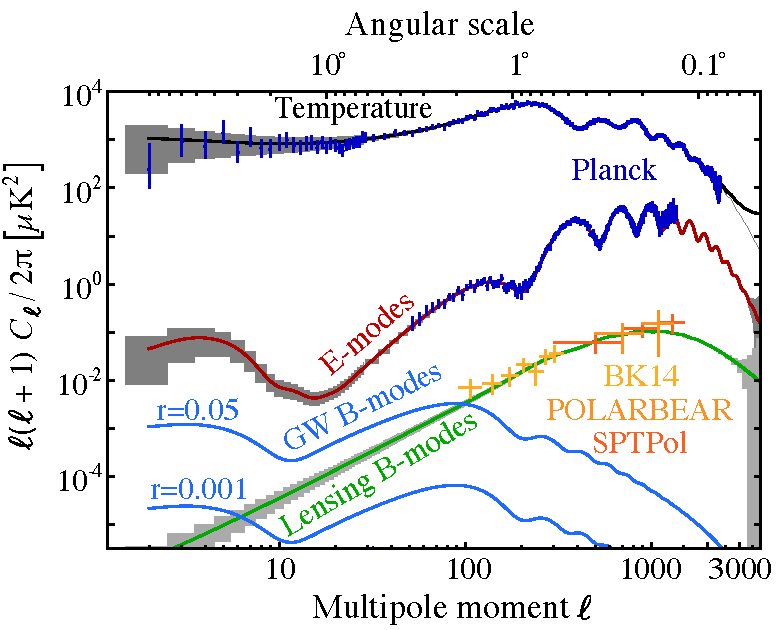
\includegraphics[width=3in]{figs/cmb_powspec_v1.pdf}  
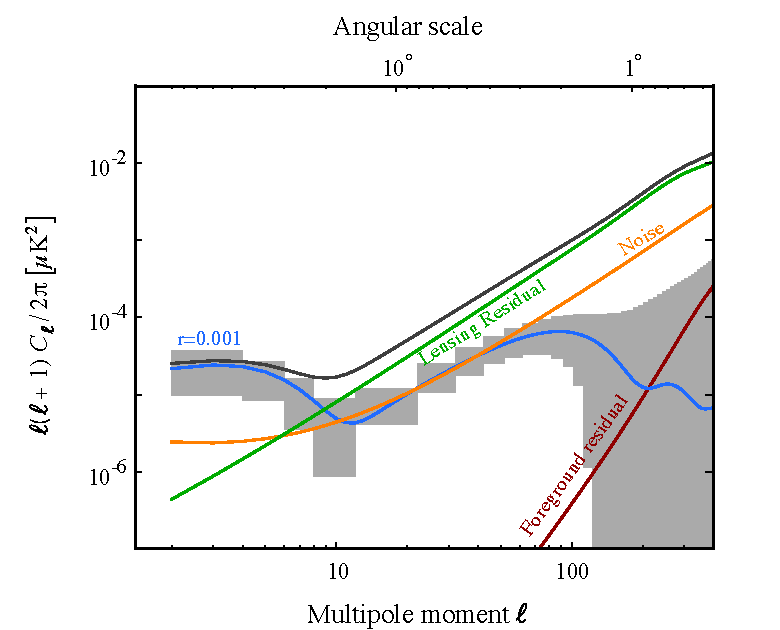
\includegraphics[width=3in]{figs/cmbbb_powspec_v1.pdf}
\end{center}
\vspace{-0.25in}
\caption{ \small \setlength{\baselineskip}{0.95\baselineskip}
Predicted determination of the \ac{CMB} power spectra for EPIC-IM (grey boxes) overlaid
on theoretical predictions (solid lines) and including Planck measurements of the 
temperature and E modes (blue) and of several ground-based measurements 
of the lensing B-modes.  The tensor B-mode predictions (blue) are shown 
for two representative values of the tensor-to-scalar
ratio: $r=0.001$ and $r=0.05.$ 
\label{fig:clall} }
\vspace{-0.05in}
\end{figure}

In slow roll Inflation there are just two observationally viable classes of models that naturally explain the measured value of the spectral index $n_s$. 
One is the set of potentials $V(\phi)\propto\phi^p$, which contains many of the canonical inflation models. This 
set is already under significant observational pressure. If the error bars on the spectral index tighten by a factor of about 2, 
and the 95\% C.L. upper limit on $r$ is pushed to even $\sim0.01$, all such models would be ruled out. 
The other class of models includes Starobinsky and Higgs inflation, which both have $r\sim0.003$. A future mission 
capable of reaching $\sigma_r\sim\mathcal{O}(10^{-4})$ would provide significant constraints on nearly every currently favored 
inflation model. The EPIC-IM configuration is forecasted to achieve \textcolor{red}{Raphael will update the following to match figures} $\sigma(r)\sim4.8 \times 10^{-4}$ assuming $r=0.001$ 
and no foregrounds.
\begin{figure}[ht!]
\parbox{4.in}{\centerline {
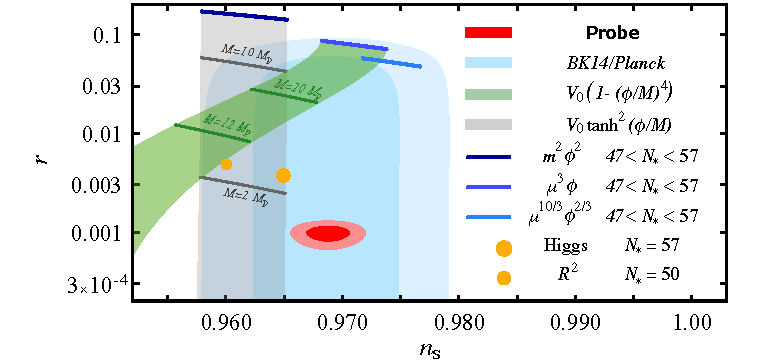
\includegraphics[width=4.5in]{figs/nsrlabeledrp001v2} } }
\hspace{-0.05in}
%\end{center}
\parbox{2.5in}{
\caption{ \small \setlength{\baselineskip}{0.95\baselineskip}
Current $1$ and $2\sigma $ limits on $r$ and $n_{s}$ (blue) and forecasted constraints for a fiducial model with $r=0.001$ for 
EPIC-IM~\cite{Array:2015xqh}. Also shown are predictions 
for the models of the inflaton potential discussed in the text: Chaotic inflation for a range of $N_\star$ values (blue lines); 
Higgs and $R^2$ (large and small dots, respectively);  quartic hilltop (green band); and a sub-class of $\alpha$-attractor
models~\cite{Kallosh:2013hoa}
\label{fig:nsrp001} } }
\vspace{-0.1in}
\end{figure}

A detection of $B$-modes consistent with a primordial spectrum of vacuum fluctuations would be the first observation 
of a phenomena directly related to quantum gravity. In addition, any detection with a next generation satellite would be 
evidence for {\it large-field} Inflation~\cite{Lyth:1996im}, in which a smooth potential that supports Inflation extends over 
a distance in field space $\Delta\phi \gtrsim M_p$. Quantum gravity studies of inflation give a generic 
expectation $\Delta\phi \lesssim M_p$~\cite{Banks:2003sx,Baumann:2014nda,Brown:2015iha,Rudelius:2015xta}, although 
there are some mechanisms to realize large-field inflation \cite{Silverstein:2008sg,Kaloper:2008fb,Marchesano:2014mla,Blumenhagen:2015xpa}. 
A detection of $r$ would therefore provide strong 
motivation to better understand how large-field inflation can be naturally incorporated into quantum gravity. 

All inflation models predict a B-mode spectrum with the shape shown in Figure \ref{fig:clall}, but inflation 
need not be correct \cite{Khoury:2001bz,Brandenberger:2012zb,Ijjas:2015hcc} and does not preclude additional sources of $B$-mode polarization either during or after 
inflation. To be confident of the implications of a detection, the shape and Gaussianity of the B-mode spectrum 
must be characterized. The vast majority of inflation scenarios predict an extremely Gaussian and nearly scale-invariant spectrum for 
gravitational waves. A target constraint of $\sigma(n_{\rm t})<1$ at $r=0.01$, driven by the information in the reionization bump, would significantly constrain non-vacuum 
inflationary sources~\cite{Namba:2015gja,Peloso:2016gqs} and rule out physics completely inconsistent with inflation. 

Deeper mapping of $E$-mode polarization will also contribute to testing inflationary models. Large scale $E$-modes will 
provide new tests of isotropy, a prediction of most models of Inflation;  
for example, the observations can reject at 99\% confidence models in which low multipoles are aligned in the temperature maps~\cite{Dvorkin:2007jp}. 
Together with continued improvements at high $\ell$ from the ground, these modes will also improve constraints on the scalar 
spectral index and its changes with scale by factors of about two. 

\begin{figure}[ht!]
\hspace{-0.2in}
\parbox{4.0in}{\centerline {
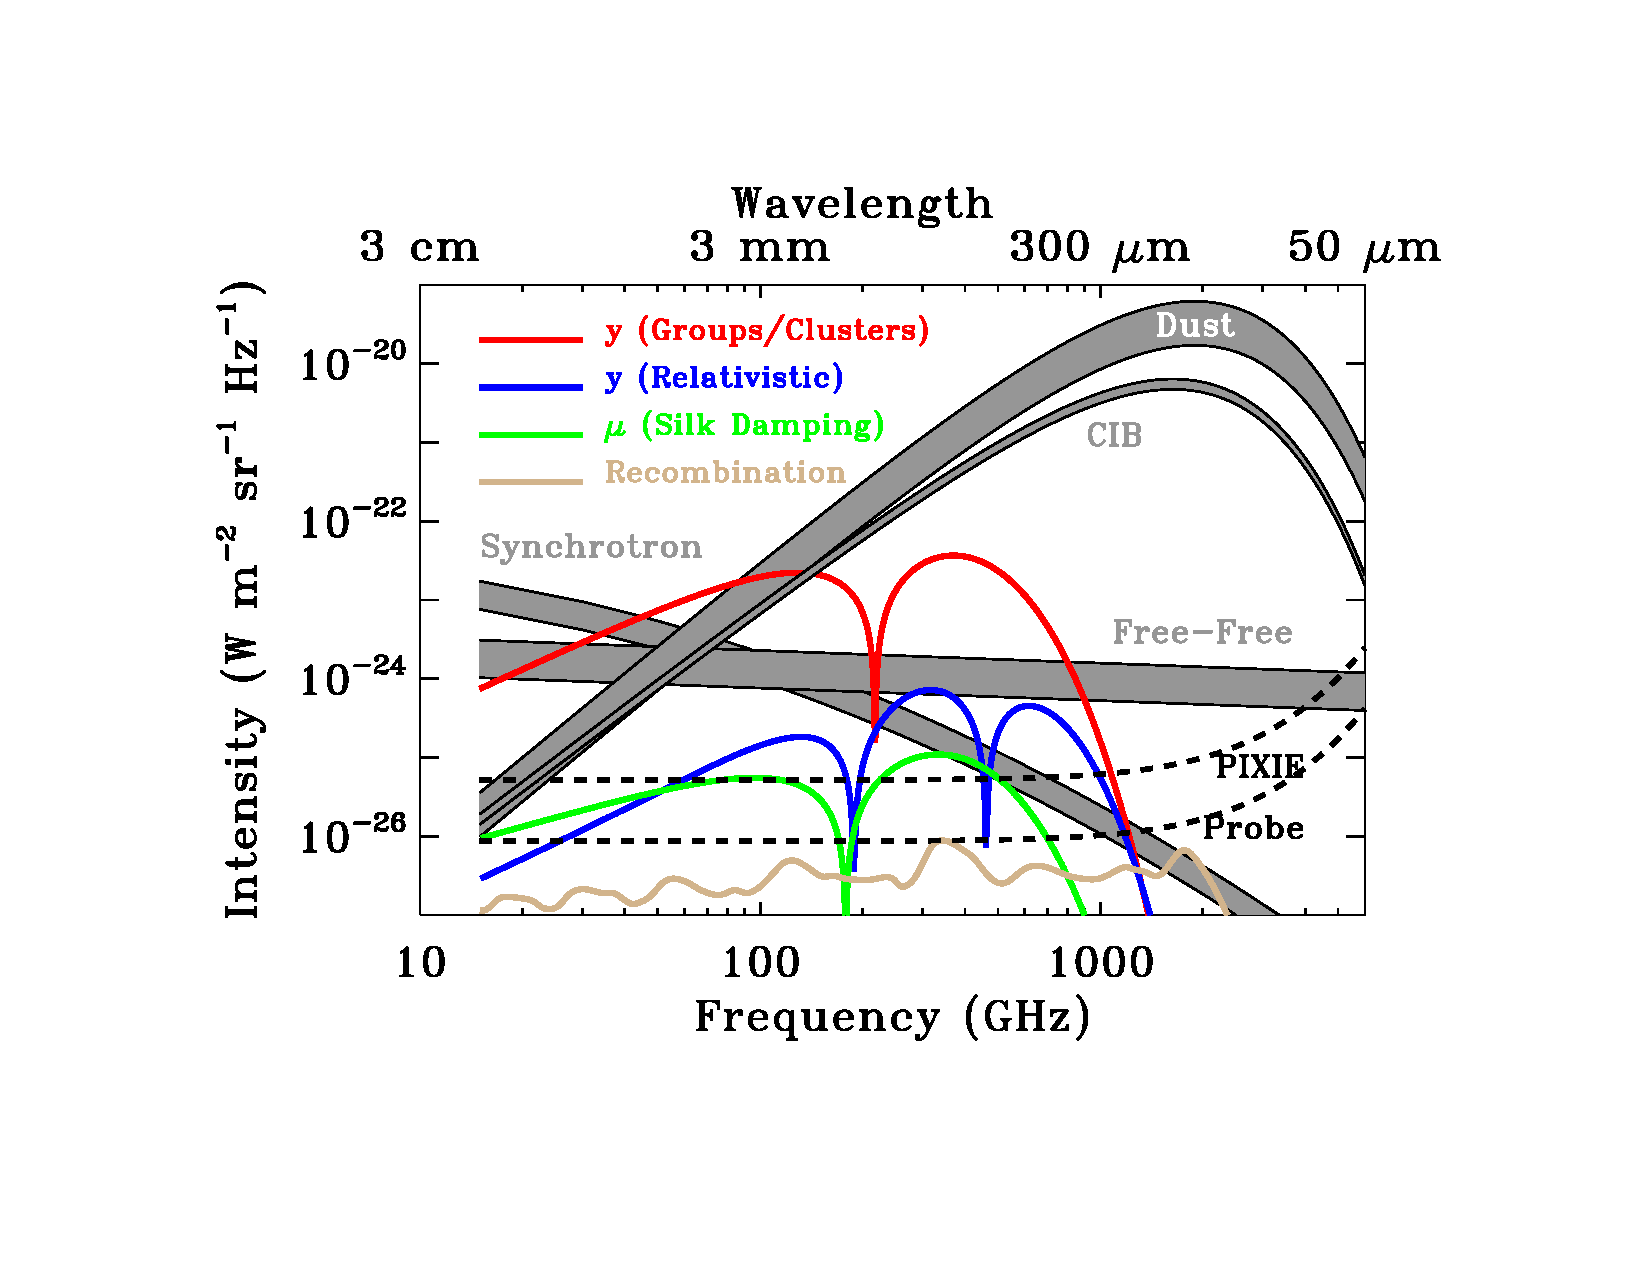
\includegraphics[width=3.0in]{Figures/probe_spectral_foregrounds_v3.pdf} } }
\hspace{-0.05in}
\parbox{2.5in}{
\caption{ \small \setlength{\baselineskip}{0.95\baselineskip}
Anticipated $y$ and $\mu$ spectral distortions (solid), the signature of resonant recombination lines (solid), and anticipated foreground 
signal levels relevant for spectral distortion measurements (grey bands). 
The simplest extension of a proposed
Explorer class mission (Probe, dash grey) gives approximately 10 times the Explorer sensitivity (PIXIE). 
A better optimized Probe may give detections of all anticipated distortions. 
\label{fig:distortions} } }
\vspace{-0.1in}
\end{figure}

Spectral distortion measurements give additional tests of Inflation. The dissipation of small-scale 
perturbations through Silk-damping leads to $\mu$-distortions~\cite{Sunyaev1970diss, Daly1991, Hu1994, Chluba2012}. 
In $\Lambda$CDM the distortions are predicted at a level of $\mu=(2.0\pm0.14)\times 10^{-8}$, a level that 
is readily accessible to a Probe class mission, see Fig.~\ref{fig:distortions}~\cite{Chluba2012, Chluba2016LCDM}. 

A better optimized probe may also give the sensitivity to detect the signature of recombination 
radiation imprinted by cosmological recombination of hydrogen and helium 
at redshift $z\simeq 10^3-10^4$; see Fig.~\ref{fig:distortions}~\citep{Sunyaev2009, Chluba2016}. 
The detailed physics is sensitive to the values of $n_{s}$, which is a direct probe of Inflation. 


%in the CMB spectrum, which provide a unique means to place stringent constraints on the amplitude of the small-scale curvature power spectrum. This information is on small scales (wavelength $0.1 \,{\rm kpc} \lesssim \lambda \lesssim 1\, {\rm Mpc}$) and from early times ($10^4 \lesssim z\lesssim 10^6$), inaccessible through any other observation. 

%In $\Lambda$CDM \citep{Chluba2012, Chluba2016LCDM}, distortions are predicted at a level of $\mu=(2.0\pm0.14)\times 10^{-8}$ (see Fig.~\ref{fig:distortions}). A detection would deliver a complementary test for the inflation paradigm~\citep{Chluba2012inflaton, Dent2012, Chluba2013PCA, Clesse2014, Cabass2016}, and new probes of the particle spectrum of inflation through new tests of non-Gaussianity~\citep{Pajer2012, Ganc2012, Biagetti2013, Razi2015, Chluba2016ng}. 
%It would also bring us to the sensitivity level required to detect the cosmological recombination radiation \citep{Sunyaev2009, Chluba2016} imprinted by the recombination of hydrogen and helium at redshift $z\simeq 10^3-10^4$, which can be used to probe the physics of recombination (see Fig.~\ref{fig:distortions}). 
%In summary, a detection of primordial gravitational waves consistent with the standard inflationary prediction would reveal the presence of a new fundamental energy scale for particle physics and would have far reaching implications for quantum gravity. Detecting correlations on the largest scales would confirm a primordial origin. Any departure from a nearly scale-invariant, nearly Gaussian spectrum would reveal new physics beyond the simplest inflationary model. In the absence of a detection, an improvement by about two orders of magnitude on the current upper limit would qualitatively change how we think about the inflationary paradigm.

\vspace{-0.15in}

\subsubsection{Light Relics and Dark Matter}

\vspace{-0.05in}

After inflation, the universe was reheated to temperatures of at least 10 MeV and perhaps as high as $10^{10}$ GeV.  
At these high temperatures, even very weakly interacting or very massive particles, such as those arising 
in extensions of the Standard model of particle physics, can be produced in large abundances~\cite{1979ARNPS..29..313S,Bolz:2000fu}.  As the universe expands and cools, 
the particles fall out of equilibrium and leave observable signatures in the \ac{CMB} power spectra. 
Through these effects the CMB is a sensitive probe of neutrino and of other particles' properties.  

One particularly compelling target is the effective number of light relic particle species $\Neff$, also called the effective 
number of neutrinos. The canonical value with three neutrino families is $\Neff = 3.046$. Additional light particles 
%in thermal equilibrium with the Standard model particles at any point in our history, it will 
contribute a change to $\Neff$ of $\Delta \Neff \geq 0.027\,g$ where $g \geq 1$ is the number of 
degrees of freedom of the new particle~\cite{Brust:2013xpv,Baumann:2016wac}.  
This defines a target of $\sigma(\Neff) < 0.027$ for future CMB observations. 
Either a limit or detection of $\Delta \Neff$ at this level would provide a powerful insight into the basic constituents 
of matter. 

Forecasts for $\Neff$ are shown in Figure~\ref{fig:Neff_future}.  The two most important parameters for improving constraints
are the fraction of sky observed $f_{\rm sky}$ and the noise. Achieving both larger $f_{\rm sky}$ and
lower noise are strengths of the CMB Probe compared to other platforms. 
Our baseline mission nearly reaches the target constraint with $g=1$, already exceeding constraints 
from other astrophysical probes and planned CMB observations.
A newly designed mission is likely to reach $\sigma(\Neff) < 0.027$ with high signal-to-noise ratio. 

\begin{figure}[t!]
\begin{center}
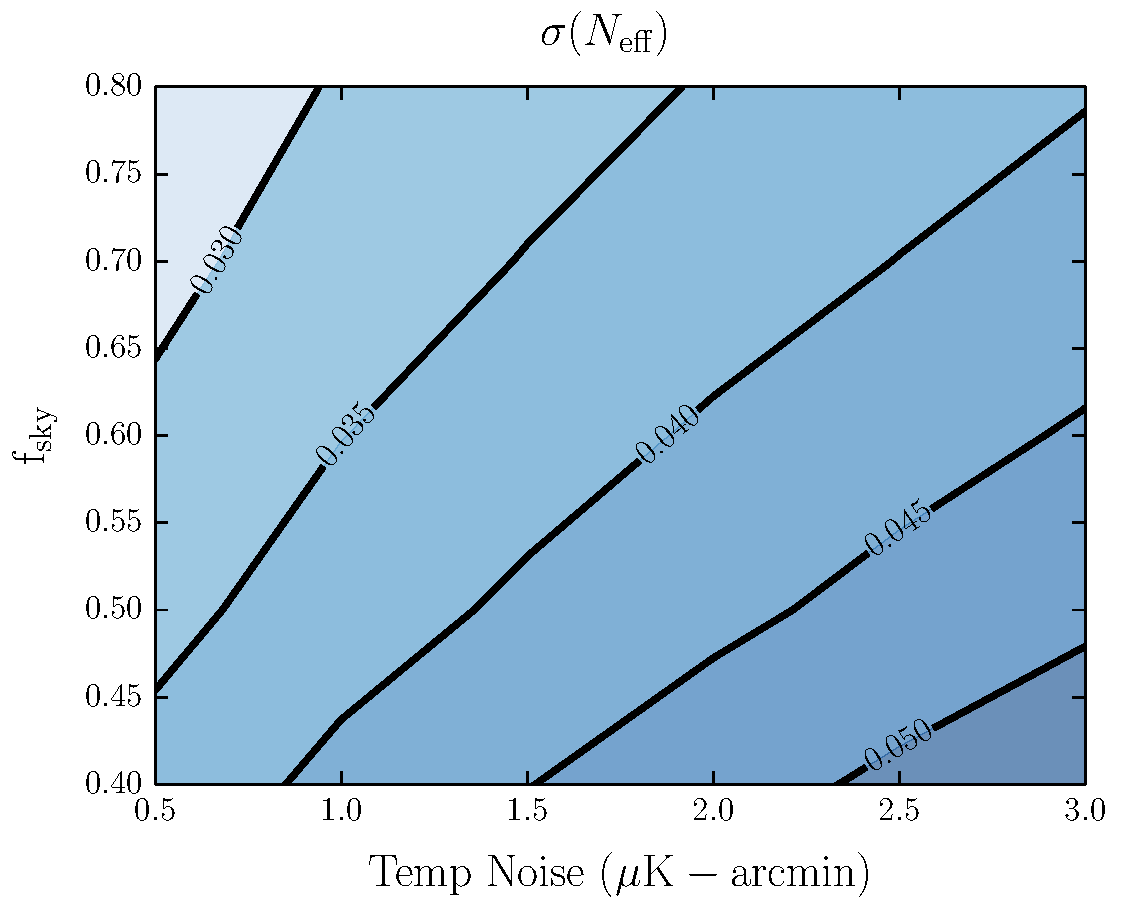
\includegraphics[width=0.45\textwidth]{figs/Neff.pdf}
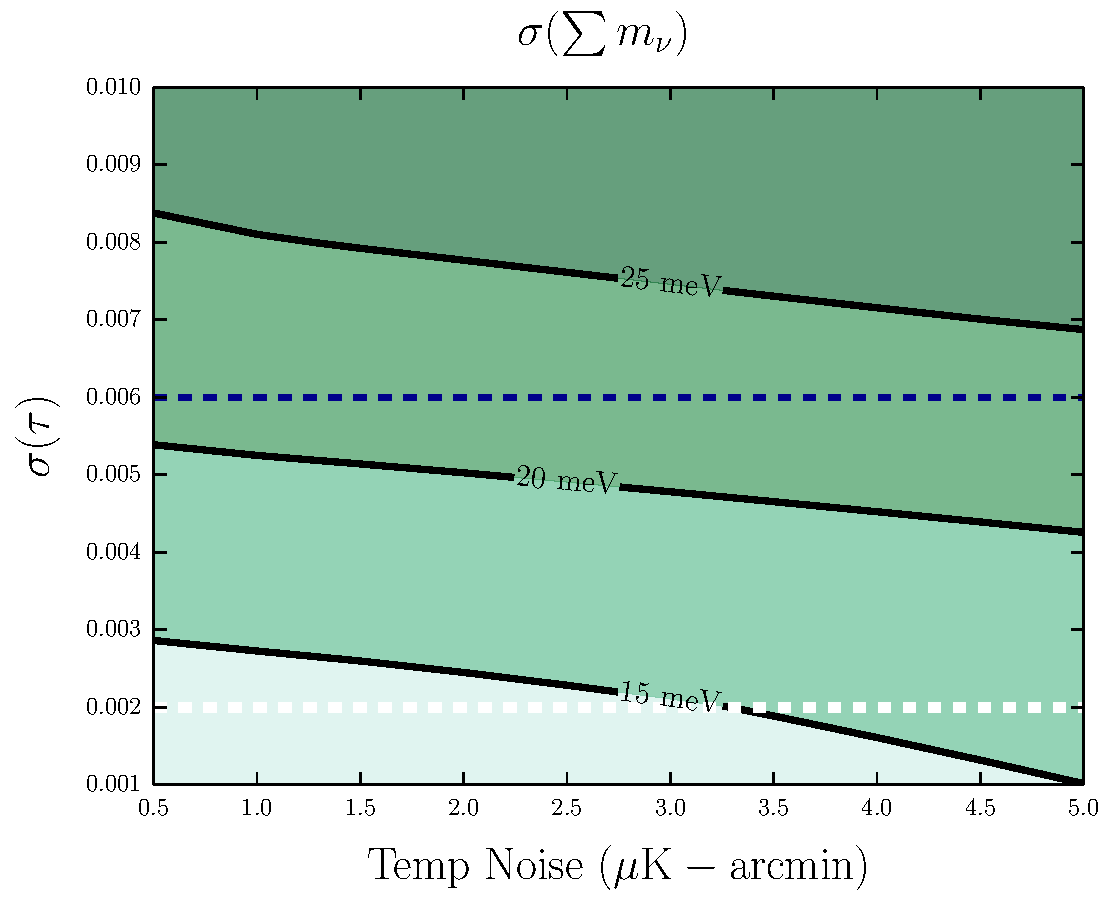
\includegraphics[width=0.45\textwidth]{figs/Mnu_tauprior.pdf}
\caption{ \small \setlength{\baselineskip}{0.95\baselineskip}
$\Neff$ as a function of noise and sky fraction (left) and
Neutrino mass constraints as a function of uncertainties in measurement of $\tau$, noise, and 
sky fraction of $f_{\rm sky} = 0.7$. The resolution assumed is 5'.  
Vertical lines denote the expected performance of EPIC-IM. 
The blue dashed line is the current \planck~limit; the grey dashed line is the limit from cosmic variance 
measurement of $\tau$. All forecasts assume internal delensing of the $T$ and $E$-maps~\cite{Green:2016cjr}, 
including residual non-Gaussian covariances.  The $\sum m_\nu$ forecasts includes DESI BAO.  
\label{fig:Neff_future} }
\end{center}
\vspace{-0.15in}
\end{figure}

Many light relics of the early universe are not stable. They decay, 
leaving faint evidence of their past existence on other tracers. The relics with sufficiently long lifetime to survive few minutes, 
past the epoch of light element synthesis, leave a signature on the helium fraction $Y_p$.  If they decay 
by the time of recombination, their existence through this period is best measured through the ratio of $\Neff$ to $Y_p$. 
The Probe's cosmic variance limited determination 
of the $E$ power spectra will improve current limits for these quantities by
a factor of five thus eliminating sub-MeV mass thermal relics. 
%  
Spectrum distortion measurements give additional constraints on the lifetime and abundance 
of such relics \citep{Sarkar1984, Kawasaki1986, Hu1993b, Chluba2011therm}. A future Probe's $\mu$-distortion constraint gives a two orders of magnitude improvement on the abundance and life time of early Universe relics \cite{Chluba2013fore, Chluba2013PCA} compared to current constraints derived from measurements of light element abundances \cite{Kawasaki2005, Jedamzik2006}.

Cosmological measurements have already confirmed the existence of one relic that lies beyond the 
Standard Model: dark matter. For a conventional WIMP candidate, the CMB places very stringent 
constraints on its properties through the signature of its annihilation on the $T$ and $E$ 
spectra \citep{Peebles2000, Chen2004, Padmanabhan2005}.  Planck currently excludes WIMPs with mass $m_{\rm dm}< 16$ GeV and a future CMB mission could reach $m_{\rm dm} < 45$ GeV for $f_{\rm sky} =0.8$.  The CMB provides the most stringent constraints on the dark matter annihilation cross section for dark matter in this mass range.  The CMB is complimentary to direct detection experiments which probe the scattering cross-section of dark matter with Standard model particles.

%A dark matter candidate can also have a slow decay to Standard models particles which is 
%similarly constrained by the CMB~\cite{Chen2004, Zhang2007, Diamanti2014, Slatyer:2016qyl}.  Current and future CMB limits on the lifetime of $\tau \gtrsim 10^{25}$ s are somewhat weaker than indirect detection limits of $\tau > 10^{24-28}$~s~\cite{Essig:2013goa}.  

A particle-independent approach is to constrain dark matter interactions that would 
affect the evolution of the effective dark matter fluid and its interactions with baryons or photons.  The simplest example is 
to constrain the baryon-dark matter cross section through its effective coupling of the two fluids~\cite{Dvorkin:2013cea}.  
These couplings affect the evolution of fluctuations and ultimately the $T$ and $E$ spectra. The current limits of $\sigma \gtrsim 10^{-31}-10^{-34}\,{\rm cm}^2 \times (m_{\rm dm} / {\rm MeV})$ can be competitive with direct detection for sub-GeV masses.  
More exotic dark sectors that include long-range forces can produce an even richer phenomenology in the CMB and in the large-scale structure 
without necessarily producing an associated signature in direct detection experiments or 
indirect searches (e.g.~\cite{Cyr-Racine:2013fsa,Buen-Abad:2015ova,Lesgourgues:2015wza}). 

Interactions of dark matter with standard model particles can also be constrained through 
measurements of spectral distortions \cite{Yacine2015DM}. 
%Chluba et al. showed 
%As the Universe expands, the matter cools. Compton interactions with electrons keep the normal matter at the CMB 
%temperature until well after recombination. This leads to a small distortion of the CMB with a negative chemical 
%potential~\citep{Chluba2011therm}. In a similar manner, interactions of DM with electron, protons or directly 
%with CMB photons can lead to a distortion. 
Current constraints from FIRAS are most sensitive to small dark matter
mass, $m_{\rm X}\lesssim 0.2\,{\rm MeV}$, but these could be extended to $m_{\rm X}\lesssim 1\,{\rm GeV}$ with a 
Probe-class mission, testing DM interaction down to cross-sections 
$\sigma\simeq 10^{-39}-10^{-35}\,{\rm cm}^2$~\cite{Yacine2015DM}. This provides new constraints on the low mass end, $m_{\rm X}\lesssim 10\,{\rm MeV}$ and improve existing limits~\cite{Essig2012PhRvL.109b1301E, Boehm2014MNRAS.445L..31B} by up to a factor of $\simeq 50$. Distortion measurements furthermore open a new avenue for testing dark matter-proton interactions~\cite{Yacine2015DM}.

A host of other physical phenomena including the existence and properties of axions, primordial magnetic fields, and 
superconducting strings, leave signatures on the spectrum of the CMB and can therefore be constrained by 
the sensitive measurements  of a future Probe~\cite[e.g.,][]{Jedamzik2000, Tashiro2012, Dolgov2013, Tashiro2013, Caldwell2013}.


\vspace{-0.15in}

\subsubsection{Neutrino Mass}

\vspace{-0.05in}

One of the last unknowns of the Standard model of particle physics is the absolute mass scale of the neutrinos.  
%While measurements of neutrino oscillations demonstrate the neutrinos have mass, directly measuring the scale of the masses is challenging experimentally.  
%Current measurement of $\Neff$ confirm the existence of a cosmological abundance of neutrinos whose gravitational influence is detectable in the CMB and in large scale structure.  
Cosmology presents a unique opportunity to measure the sum of neutrino masses $\sum m_\nu$ through the 
suppression of the growth of structures in the Universe on small scales.  
%Larger $\sum m_\nu$ gives a larger suppression and the $\sum m_\nu$ can be measured by 
%The \ac{CMB} Probe would be a valuable tool in the quest for a cosmological detection of $\sum m_\nu$.   
The sensitivity to $\sum m_\nu$ from suppression of power is limited by our knowledge of 
the primordial amplitude of fluctuations $A_s$, which is strongly degenerate with the optical depth $\tau$.  
The current limit on $\tau$ from \planck\ of $\sigma({\tau}) = 0.009$~\cite{} limits 
$\sigma(\sum m_\nu) \gtrsim 25$ meV. Forcasts for an internal 
CMB measurement of $\sum m_\nu$ via CMB lensing~\cite{Kaplinghat:2003bh} are shown Figure~\ref{fig:Neff_future} but the conclusion is the same for any proposed cosmological probe.
%This lower limit is common to any measurement that depends on the relative suppression.  
Therefore, a cosmological detection of the minimum value expected from particle physics  
$\sum m_\nu = 58$~meV at more than $2 \sigma$ will require a better measurement of $\tau$.  
The best constraints on $\tau$ come from $E$-modes with $\ell < 20$ which require 
measurements over the largest angular scales.
To date, the only proven method for such a measurement is from space.  
The \ac{CMB} Probe will reach the cosmic variance limit of $\tau \sim 0.002$ and will therefore 
reach $\sigma(\sum m_\nu) < 15$ meV when combined with DESI's measurements of 
baryon acoustic oscillations~\cite{Levi:2013gra}.  
A detection of $\sum m_\nu$ at this level is not possible with any other existing survey.
%if not accompanied by an improvement to the measurement of $\tau$.

\vspace{-0.15in}

\subsubsection{Cosmological structure formation}

\vspace{-0.05in}

Understanding the evolution of cosmological structures from small density perturbations through the formation of the
first stars to present day galaxies and cluster is a key goal of cosmology~\cite{dunlop2011}. 
Cosmological reionization, the transition of the Universe from dominated by neutral to ionized 
hydrogen, is a cornerstone of this evolution because it encodes information 
about the star formation history and the physical processes that formed the galaxies of various luminosities and masses we see today. 
But when did the epoch of reionization start?  How long did it last? Are early galaxies enough to reionize the entire Universe
or is another source required?
 
Measurements of the \ac{CMB} $E$ mode power spectrum over large angular scales are sensitive to the optical depth 
to reionization $\tau$, a key parameter for all reionization models that attempt to answer these questions. 
The \planck\ team  reported recently a value of $\tau=0.055 \pm 0.009$~\cite{planck2016_xlvi,planck2016_xxxi}.
The level is significantly lower than previous estimates and reduces the tension between CMB-based analyses and constraints from 
other astrophysical sources.  
%While the average redshift at which reionization occurs is found to be $z_re\simeq 8$ assuming an 
%instantaneous reionization, suggesting that reionization occurred rather late.
The CMB Probe's cosmic variance limited measurement of $E$-mode polarization will 
improve the $1\sigma$ error by a factor of 4.5 to reach a cosmic 
variance limited measurement of $\tau$, thus setting 
stringent constraints on models of the reionization epoch. 
% that require additional sources of reionization, non-standard early galaxies, 
%or significantly evolving escape fractions or clumping factors. On the whole a better estimate of $\tau$ when combined with direct probes at low redshift, 
%will help to characterize the duration of the epoch of reionization and tell us when it started.

%will  set stringent constraints on models of the reionization epoch. \comred{what is the quantitative connection to models of reionization}.

%The optical depth to reionization, $\tau$, places an important integral constraint on the extended reionization history.
%The {\it Planck} Collaboration~\cite{planck2015-XLVI,planck2015-XXXI} reported recently a value of $\tau=0.055 \pm 0.009$ significantly lower than previous estimates. 
%This suggests that an early onset of reionization is strongly disfavoured by the {\it Planck} data. 
%The {\it Planck} Collaboration~\cite{planck2015-XXXI} showed that this result reduces the tension between CMB-based analyses and constraints from 
%other astrophysical sources. 
%A cosmic variance limited measurement of E-mode polarization on large scales, possible with a probe mission, will render the most accurate 
%determination of $\tau$ (Figure~\ref{fig:Neff_future}
%shows a cosmic variance limit measurement of $\tau$ along with the current {\it Planck} limit, break the degeneracy with the neutrino mass, 
%set stringent constraints on models of the reionization epoch, and, finally, help understanding the formation of the cosmological structures we see today.

The anisotropy in the \ac{CIB} produced by dusty star-forming galaxies in a wide redshift range, are
an excellent probe of both the history of star formation and the link between
galaxies and dark matter across cosmic time. The \planck\ collaboration 
derived values of the star formation rate that,
at redshifts z$\mathrm{\sim3}$, are three times larger 
than constraints from number counts measurements (\cite{planck2014-XXX,planckXVIII,madau2014}).
The new mission probe, 
By measuring \ac{CIB} anisotropy with 100 times higher signal-to-noise ratio
the CMB Probe will shed light on this intriguing discrepancy. 
Specifically, it will constrain the star formation rate with one tenth of \planck 's uncertainty. 


A key parameter in simulations of the angular power spectrum of the \ac{CIB} 
is $M_{\mathrm{eff}}$, the galaxy hallo mass that is most efficient in producing star 
formation activity. Comparing measurements of the power spectrum to simulations
constrains this parameter, which informs structure formation models. Current models and measurements 
find $M_{\mathrm{eff}}\sim 10^{12}$ solar masses with about $\mathrm{10\%}$ uncertainty. 
The CMB Probe will constrain this parameter at the percent level.


%Dusty star-forming galaxies trace the underlying dark matter
%field in a broad redshift range. Therefore, a wealth of information will be extracted by 
%correlating the anisotropy in the \ac{CIB} 
%with multiple dark matter tracers including catalogs of galaxies and quasars, 
%and maps of the $\gamma$-ray and the X-ray background~\cite{serra2014,wang2015,cooray2016}.
%These cross-correlations will provide an additional probe of the star formation history, and they will shed light on the interaction between 
%light and matter in a broad wavelength range. \comred{the paragraph starts with dark matter, but ends 
%with SFR ..?}

The transition to reionized Universe and the onset of structure formation inject
energy into the sea of CMB photons. This injection is detectable through a distinct spectral distortion. 
This is the largest expected distortion -- marked `$y$ Groups/Clusters' in Figure~\ref{fig:distortions} --
and will be clearly detected by the CMB Probe. 
A detection will give information about the total energy output of the first stars, AGNs, and galaxy clusters, 
an important parameter in structure formation models. 

Group-size clusters that have masses $M\simeq 10^{13}\,M_{\odot}$ contribute significantly to the signal. 
With temperature $k T_{\rm e}\simeq 1\,{\rm keV}$ these are sufficiently hot to create a relativistic 
temperature correction to the large $y$-distortion. This relativistic correction, denoted `$y$ relativistic' in 
Figure~\ref{fig:distortions},  will also be detected with high signal-to-noise ratio by the CMB Probe, and 
will be used to constrain the currently uncertain feedback mechanisms used in hydrodynamical simulations
of cosmic structure formation~\citep{Hill2015}. 

%Large-scale structure can also be probed using CMB spectral distortions measurements. 
%In fact, the largest guaranteed distortion is caused by the associated late-time energy release of 
%forming structures and from reionization~\cite{Sunyaev1972b, Hu1994pert, Oh2003, Cen1999, Refregier2000}, 
%imprinting a $y$-type distortion with $y \simeq 2\times 10^{-6}$ \citep[e.g.,][]{Refregier2000, Hill2015}. 
%This distortion is only one order of magnitude below the current limit from COBE/FIRAS and, even with most 
%pessimistic assumptions about foregrounds, should be clearly detected with the next-generation spectrometers we propose to study. 
%A detection will give information about the total energy output of first stars, AGN and galaxy clusters. \comred{what do 
%you do with this number? how does this feedback to constraints on SFR or other parameters of structure evolution models?}
%In particular, group-size clusters that have masses $M\simeq 10^{13}\,M_{\odot}$ contribute significantly to the signal. 
%With temperature $k T_{\rm e}\simeq 1\,{\rm keV}$ these are sufficiently hot to create a relativistic 
%temperature correction to the large $y$-distortion. This relativistic correction, denoted `$y$ relativistic' in 
%Figure~\ref{fig:distortions},  
%which can be used to constrain the currently uncertain feedback mechanisms used in hydrodynamical simulations
%of cosmic structure formation~\citep{Hill2015}.  (see Fig.~\ref{fig:distortions}).

The CMB spectrum varies spatially across the sky. One source of such anisotropic distortion is due to 
the spatial distribution clusters of galaxies and has already been measured by Planck~\cite{Planck2013SZ}. 
A combination of precise CMB imaging 
and spectroscopic measurements will allow observing the relativistic temperature correction of individual SZ 
clusters~\cite{Sazonov1998,Itoh98,Challinor98}, which will calibrate cluster scaling relations and inform our 
knowledge of the dynamical state of the cluster atmosphere. 

Resonant scattering of the CMB photons during and post last scattering leads to spectral-spatial signals
that can be used to constrain the abundance of metals in the dark ages and therefore the make-up of the 
first, and subsequent generations of stars~\cite{Jose2005, Carlos2007Pol, Lewis2013,Kaustuv2004, Schleicher2008}. 
